\documentclass[12pt, twoside]{article}
\input{/Users/chris/github/course-files/docs/ib/preamble}

\fancyhead[LO]{La Scuola d'Italia / Dr.\ Huson / IB Math 12 HL \\* 29 September 2026}
\fancyhead[RO]{\fbox{\begin{minipage}{6cm}\footnotesize Nickname:\\[0.5cm]\end{minipage}}}
\fancyhead[LE]{\fbox{\begin{minipage}{6cm}\footnotesize Nickname:\\[0.5cm]\end{minipage}}}
\fancyfoot[C]{\thepage}

\begin{document}
\subsubsection*{12.5 Classwork: Roots of Complex Numbers (no calculator)}

Answer all four problems in the spaces provided. Show your working. Give all
answers as exact values (surds and fractions of $\pi$), not decimals.

\begin{enumerate}[itemsep=0.15cm]

%--- Problem 1: Square roots of 5 - 12i in Cartesian form; complex quadratic; why not a conjugate pair [6 marks] ---
%--- Source: authored 2026-09-29 (HL syllabus 1.12, 1.14; review of 12-2CW) ---
\item[1.]

\begin{enumerate}[itemsep=0.15cm]
  \item By writing $(a + bi)^{2} = 5 - 12i$, where $a, b \in \mathbb{R}$,
  find the two square roots of $5 - 12i$.
  \item Hence solve the equation
  $$z^{2} - 2z - 4 + 12i = 0.$$
  \item Explain why the two solutions in (b) are not a conjugate pair.
\end{enumerate}

\begin{tikzpicture}
  \draw (-0.6,0) rectangle (14.6,15.8);
  \foreach \y in {1,2,...,15} \draw[dotted] (0,\y)--(14.1,\y);
\end{tikzpicture}

\newpage

%--- Problem 2: Fourth roots of -8 + 8sqrt3 i; Cartesian form; conjugate equation [7 marks] ---
%--- Source: authored 2026-09-29 (HL syllabus 1.13, 1.14) ---
\item[2.]

Let $w = -8 + 8\sqrt{3}\,i$.

\begin{enumerate}[itemsep=0.15cm]
  \item Write $w$ in the form $re^{i\theta}$, where $r > 0$ and
  $-\pi < \theta \leq \pi$.
  \item Solve the equation $z^{4} = w$, giving each solution in the form
  $re^{i\theta}$, where $r > 0$ and $-\pi < \theta \leq \pi$.
  \item Write the solution that lies in the first quadrant in the form
  $a + bi$.
  \item Hence write down the four solutions of
  $z^{4} = -8 - 8\sqrt{3}\,i$, in the form $re^{i\theta}$.
\end{enumerate}

\begin{tikzpicture}
  \draw (-0.6,0) rectangle (14.6,16.4);
  \foreach \y in {1,2,...,15} \draw[dotted] (0,\y)--(14.1,\y);
\end{tikzpicture}

\newpage

%--- Problem 3: Cube roots of unity; hence (z - 1)^3 = 8; real factorization of the cubic [6 marks] ---
%--- Source: authored 2026-09-29 (HL syllabus 1.14; review of 12-2CW polynomial roots) ---
\item[3.]

\begin{enumerate}[itemsep=0.15cm]
  \item Find the three cube roots of $1$, giving each in the form $a + bi$.
  \item Hence solve the equation $(z - 1)^{3} = 8$, giving each solution in
  the form $a + bi$.
  \item Show that the equation in (b) can be written as
  $z^{3} - 3z^{2} + 3z - 9 = 0$. Hence write $z^{3} - 3z^{2} + 3z - 9$ as
  the product of a linear factor and a quadratic factor with real
  coefficients.
\end{enumerate}

\begin{tikzpicture}
  \draw (-0.6,0) rectangle (14.6,17.4);
  \foreach \y in {1,2,...,16} \draw[dotted] (0,\y)--(14.1,\y);
\end{tikzpicture}

\newpage

%--- Problem 4: Given one cube root 1 + sqrt3 i, find w and the other roots; triangle area [6 marks] ---
%--- Source: authored 2026-09-29 (HL syllabus 1.13, 1.14; review of 12-3CW de Moivre) ---
\item[4.]

One of the cube roots of the complex number $w$ is $1 + \sqrt{3}\,i$.

\begin{enumerate}[itemsep=0.15cm]
  \item Use de Moivre's theorem to find $w$.
  \item Find the other two cube roots of $w$, giving each in the form
  $a + bi$.
  \item The three cube roots of $w$ are plotted on an Argand diagram. Find
  the exact area of the triangle they form.
\end{enumerate}

\begin{center}
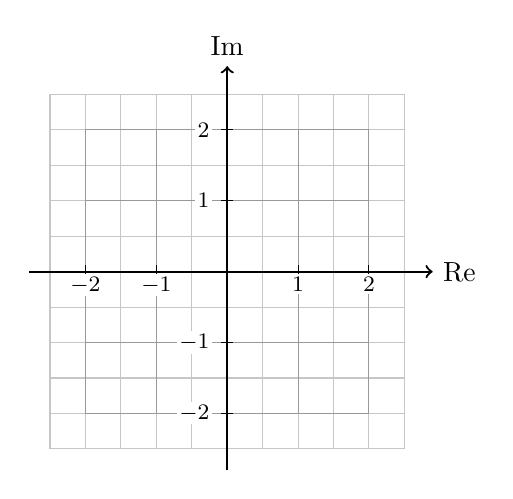
\begin{tikzpicture}[scale=0.9]
  \draw [thin, color=gray!45, step=0.5cm] (-2.5,-2.5) grid (2.5,2.5);
  \draw [thin, color=gray!80] (-2,-2) grid[step=1cm] (2,2);
  \draw [thick, ->] (-2.8,0) -- (2.9,0) node [right] {$\mathrm{Re}$};
  \draw [thick, ->] (0,-2.8) -- (0,2.9) node [above] {$\mathrm{Im}$};
  \foreach \x in {-2,-1,1,2} \draw[shift={(\x,0)}] (0pt,-2.5pt) -- (0pt,2.5pt)
     node[below=3pt, fill=white, inner sep=1pt] {\footnotesize $\x$};
  \foreach \y in {-2,-1,1,2} \draw[shift={(0,\y)}] (2.5pt,0pt) -- (-2.5pt,0pt)
     node[left=3pt, fill=white, inner sep=1pt] {\footnotesize $\y$};
\end{tikzpicture}
\end{center}

\begin{tikzpicture}
  \draw (-0.6,0) rectangle (14.6,11.4);
  \foreach \y in {1,2,...,10} \draw[dotted] (0,\y)--(14.1,\y);
\end{tikzpicture}

\end{enumerate}
\end{document}
